%% vim:ft=tex
\documentclass[font=plain,chapter=TITLE,section=Title,espaco=duplo,tocpage=plain,appendix=Name,floatnumber=continuous]{abnt}
\usepackage{hyperref}
\usepackage[utf8]{inputenc}
\usepackage[brazil]{babel}
\usepackage[alf]{abntcite}
\usepackage{graphicx}
\usepackage{timestamp}
\usepackage{amssymb,amsmath}

%% xunxo para seguir as normas da UTP
\usepackage{xunxos-utp}

%% informações sobre o trabalho
\autor{Bogdano Arendartchuk}
\titulo{Avaliação de técnicas de predição de comportamento de máquinas
virtuais para a otimização de uso de parque computacional}
\comentario{Trabalho de Conclusão de Curso apresentado ao Curso de Bacharelado
em Ciência da Computação, da Faculdade de Ciências Exatas da Universidade
Tuiuti do Paraná, como requisito parcial para a obtenção do grau de Bacharel em
Ciência da Computação.}
\instituicao{Universidade Tuiuti do Paraná}
\orientador[Orientador: ]{Islenho Almeida}
\local{Curitiba}
\data{2010}

\begin{document}
%% xunxos-utp.sty
%% Copyright 2010 Bogdano Arendartchuk <bhdn@ukr.net>
%
% This work may be distributed and/or modified under the
% conditions of the LaTeX Project Public License, either version 1.3
% of this license or (at your option) any later version.
% The latest version of this license is in
%   http://www.latex-project.org/lppl.txt
% and version 1.3 or later is part of all distributions of LaTeX
% version 2005/12/01 or later.
%
% This work has the LPPL maintenance status `maintained'.
% 
% The Current Maintainer of this work is M. Y. Name.
%
% This work consists of the files xunxos-utp.sty and xunxos-utp-doc.tex.
%
\renewcommand{\figurename}{FIGURA}
\renewcommand{\tablename}{TABELA}
\citeoption{minhasopcoes}
\nohyphens


\UTPCapa
\UTPFalsaFolhaDeRosto
\UTPFolhaDeRosto

\begin{resumo}
Este trabalho apresenta uma metodologia de um sistema de predição de
comportamento de máquinas virtuais em um ambiente gerenciado pela
ferramenta libVirt. São estudadas as técnicas de aprendizado Máquinas de
Vetores de Suporte e $k$ Vizinhos mais Próximos, além dos conceitos e
ferramentas relacionados a virtualização. Por fim são apresentados os
modelos, processos e técnicas que serão utilizados no sistema, bem como um
cronograma das atividades previstas.

Palavras-chave: virtualização; aprendizado de máquina; libVirt; Linux; SVM
\end{resumo}

\listoffigures
%\listoftables
\listadequadros
\sumario

% definições globais para o trabalho

\newcommand{\libvirt}{\emph{libVirt}}


%
% Introdução
%

\chapter{Introdução}

Com a crescente disponibilização de aplicações por meio da Internet, ter
recursos computacionais (processamento, armazenamento, entre outros)
resilientes para prover as mesmas é cada vez mais um requisito. Assim,
empresas que oferecem estes recursos como forma de serviço, geralmente
empresas de hospedagem de \emph{websites} e aplicações, precisam adotar
tecnologias de alta disponibilidade em seus ambientes computacionais.

Neste contexto, as tecnologias de virtualização possibilitam que um ou mais
sistemas computacionais sejam executados dentro de um outro sistema,
permitindo, assim, que o estado destes possa ser controlado por uma aplicação
externa, chamada também de hipervisor, que pode prover serviços de
alta disponibilidade desses sistemas, comumente chamados de máquinas
virtuais. Pode-se, por exemplo, migrar uma máquina virtual que está
executando em um computador para outro ou mesmo mudar sua configuração,
como quantidade de memória RAM, sem que este processo resulte em uma
interrupção prejudicial ao serviço disponibilizado.

Produtos como \emph{VMware,}\footnote{http://www.vmware.com}
\emph{Xen,}\footnote{http://xensource.com/}
\emph{Virtualbox}\footnote{http://virtualbox.org/} e
\emph{KVM}\footnote{http://linux-kvm.org/} (desenvolvidos por VMware,
Citrix, Oracle e Red Hat, respectivamente) oferecem ferramentas para a
execução e manutenção de máquinas virtuais. Além disso, esses produtos
proveem APIs (\emph{Application Programming Interface}, Interface para Programação
de Aplicações) que permitem que terceiros desenvolvam aplicações
específicas que gerenciem essas máquinas virtuais ou coletem informações a
respeito das mesmas. Para abstrair as diferenças entre cada API de cada
fornecedor, a biblioteca \libvirt{} oferece uma API uniforme para gerenciar
máquinas virtuais independente de qual produto de virtualização é
utilizado.

Tendo alta disponibilidade, esses provedores de recursos computacionais
precisam, também, tentar fazer bom uso de seu parque de computadores
disponíveis, minimizando custos de manutenção e energia elétrica,
sem degradar a qualidade do que é provido aos clientes. Mantendo mais
máquinas virtuais em um mesmo hipervisor diminui custos de energia e
manutenção, tendo porém, o risco de degradar o desempenho, uma vez que
unidades de processamento (CPUs) e barramentos de dados são utilizadas
concorrentemente entre as máquinas virtuais.

Com isso, fica evidente o potencial de aproveitar as ferramentas e APIs de
virtualização para observar o comportamento de máquinas virtuais de maneira
a tentar prever quando é mais adequado separar máquinas virtuais ou
agrupá-las\footnote{Entende-se agrupamento simplesmente por
executar máquinas virtuais em um mesmo computador, independente do
\emph{software}
que está executando dentro dessas máquinas. Porém, o caso mais comum em
ambientes comerciais trata-se de servidores de aplicações web e banco de
dados.} em um mesmo computador. 

Assim, este trabalho apresenta um \emph{software} que utiliza técnicas de
aprendizado de máquina para prever o comportamento de máquinas
virtuais em um ambiente de virtualização baseado em \libvirt{}, tendo como
objetivo a minimização (consolidação) do uso de recursos usados em parque
computacional, quando possível. São avaliadas as técnicas de Máquinas de
Vetores de Suporte e $k$-NN para a predição e a técnica de \emph{first fit} para
a alocação. Para avaliar a metodologia é utilizado um histórico de uso de CPU
em um ambiente de compilação de \emph{software} que faz parte do projeto \emph{Mandriva
Linux\footnote{http://www.mandriva.com/}}.

Na seção \ref{sec:aprendizado} é apresentado o conceito de aprendizado de
máquina, com uma descrição detalhada de Máquinas de Vetores de Suporte na seção
\ref{sec:svm}. A seção \ref{sec:relacionados} apresenta trabalhos com objetivos
e/ou técnicas relacionadas.Os conceitos relacionados às tecnologias de
virtualização são descritos na seção \ref{sec:virt}, com uma descrição à
ferramenta \libvirt{} na seção \ref{sec:libvirt}. Então é apresentada a
metodologia de desenvolvimento do projeto na seção \ref{sec:meto}. Finalmente,
na seção \ref{sec:resultados} são apresentados os testes realizados e resultados
obtidos.


%
% Revisão da Literatura
%

\chapter{Revisão da literatura}

\section{Aprendizado de Máquina}\label{sec:aprendizado}

% 
% Aprendizado de máquina
%

%%%%%%
% TODO verificar os TODO e os FIXME antes da próxima" "release"
%%%%%%

\newcommand{\vect}[1]{\mathbf{#1}}
\newcommand{\norma}[1]{\lVert #1 \rVert}

% Usar Inductive Principles for Learning from Data como referência "dos
% tópicos" para esse assunto, e também o "Uma Introdução às Support Vector
% Machines".
% Tomar cuidado em manter a consistência entre as diferentes notações
% usadas entre as referências.
%
% - A teoria do aprendizado estatístico
% - Métodos paramétricos
% - Métodos adaptativos
% - Risco esperado, risco estatístico
% - Classificação binária
% - Classificação multi-classes
% - Como adaptar um classificador binário para um problema multi-classes
%   (Pairwise, e esqueciooutro)
%
% Apresentar (brevemente) algumas outras técnicas também:
% (lista baseada em wiki/Supervised_learning#Approaches_and_algorithms)
% - redes neurais artificiais
% - inferência bayesiana
% - ...
%
% FIXME Aqui realmente estou em dúvida. Devemos apresentar TODAS as
% técnicas, uma por parágrafo, ou apresentar uma a uma?
% -- Pelo que tenho visto em outras monografias, não é necessário
%  apresentar o estado da arte da área de aprendizado (Ver Trabalhos
%  Relacionados no Google Docs)

Um dos comportamentos mais característicos de sistemas computacionais que possam ser considerados inteligentes é o de melhorar o seu desempenho para resolver algum problema quando este se depara com a mesma situação por mais de uma vez ~\cite{luger2004inteligencia}. ~\apudonline{simon1983should}{luger2004inteligencia} define o conceito de aprendizado de máquina como sendo qualquer mudança que melhore o seu desempenho na segunda vez que ele repetir a mesma tarefa, ou em uma tarefa da mesma população.

Nem sempre é possível obter um resultado ótimo para novas situações, pois na maioria dos casos não é possível apresentar a um sistema a quantidade de exemplos (ou experiências anteriores) necessárias para representar todos os casos possíveis. Por isso, as técnicas de aprendizado fazem uso da inferência indutiva, que consiste em prever novas situações baseando-se em um conjunto particular de exemplos~\cite{luger2004inteligencia}.

A construção da hipótese no aprendizado indutivo ocorre por meio da exposição de exemplos ao algoritmo de indução, sendo este processo chamado de treinamento. O processo de atribuir rótulos ou classes a novos exemplos é chamado de classificação. Porém, se o conjunto de exemplos usado para a indução for muito pequeno ou pouco representativo, há o risco de que as hipóteses escolhidas não descrevam corretamente novas situações e o sistema inteligente traga resultados incorretos~\cite[p. 90]{rezende2003sistemas}.

Sistemas de aprendizado de máquina podem ser divididos em dois tipos, dependendo de como são realizadas suas respectivas etapas de treinamento: supervisionados e não-supervisionados.

O aprendizado supervisionado é aquele em que há exemplos pré-existentes e estes já possuem rótulos. Tais rótulos podem ter sido atribuídos por um especialista no domínio ou representam resultados de experiências anteriores do sistema. Um classificador baseado em aprendizado supervisionado deve tentar estabelecer uma hipótese que seja genérica a ponto de que o algoritmo possa classificar corretamente novos casos. Uma hipótese muito genérica pode resultar em uma classificação inadequada (\emph{underfitting} --- sub-ajuste), ao passo que uma hipótese que descreva corretamente apenas os exemplos que foram usados para o treinamento pode ter um desempenho inadequado em casos novos (\emph{overfitting} --- sobre-ajuste).

No aprendizado não-supervisionado, não há rótulos para atribuir aos exemplos, pois o objetivo do algoritmo é encontrar grupos de exemplos que possuam semelhança entre eles. As técnicas deste modelo são referenciadas como sendo ``técnicas de agrupamento'' ou \emph{clustering}~\cite{rezende2003sistemas}.
%FIXME terminar não-supervisionado (dar uma olhada no livro do Luger)

\subsection{Técnicas de aprendizado supervisionado}

Dentre as técnicas de aprendizado supervisionado mais populares estão, não exclusivamente supervisionados, Redes Neurais Artificiais, Máquinas de Vetores de Suporte (SVMs --- \emph{Support Vector Machines}), $k$ Vizinhos Mais Próximos ($k$-NN --- \emph{k-Nearest Neighbors}) e \emph{Naïve Bayes}.

% FIXME faltou descrever GGM, RBF, Redes Bayesianas e árvores de decisão

$k$-NN é uma técnica de aprendizado supervisionado que utiliza todos os exemplos durante a etapa de classificação, tendo assim pouco custo para treinamento e alto custo para classificação. Para classificar as entradas, comumente mede-se a distância euclideana de todos os exemplos da base e então é selecionada a classe que predomina no grupo de $N$ elementos que estiver mais próximo\cite{tan2006effective}.

Há também as técnicas baseadas em Árvores de Decisão, que visam a indução de uma árvore que represente o conhecimento. Os ramos desta árvore indicam conjunções (tanto de testes binários quanto multivalorados), ao passo que as folhas representam classficações. Para classificar novos casos simplemente percorre-se a árvore de decisão avaliando cada conjunção em cada ramo e seguindo para a subárvore adequada, quando atinge-se as folhas é encontrada a classe final~\cite{de-categorizacao}. Esta técnica possui a vantagem de que sua forma de representação permita que humanos compreendam com facilidade o conteúdo que ela representa~\cite[p. 52]{mitchell1997machine}. Os algoritmos para indução de árvores de decisão mais populares são ID3~\cite{quinlan1986induction}, C4.5~\cite{quinlan1993programs} e CART~\cite{breiman1984classification}.

\emph{Naïve Bayes} é um algoritmo de aprendizado supervisionado, que
utiliza probabilidade para a classificação, supondo que as variáveis de cada
exemplo são condicionalmente independentes \cite{de-categorizacao}, as
probabilidades são calculadas de acordo com o Teorema de Bayes
\cite{kim2003poisson}, para a classificação de um elemento desconhecido, é
calculada a probabilidade de todas as classes e a classe com maior
probabilidade é escolhida como rótulo para o elemento desconhecido.
~\cite{pardo2002aprendizado}

A técnica de Redes Neurais Artificiais (RNAs) baseou-se originalmente no comportamento de neurônios observados na natureza. Uma RNA é formada por uma rede com grande quantidade de unidades de aprendizado, que recebem uma série de valores contínuos que fazem parte dos exemplos de treinamento, produzindo então um valor contínuo, que por sua vez pode ser repassado para outros agrupamentos dessas unidades ou ser utilizado para reajustar pesos internos, permitindo que novos exemplos sejam classificados em iterações futuras.~\cite[p. 81-86]{mitchell1997machine}

SVMs é uma técnica modelada como um problema de otimização que tenta encontrar, no espaço do conjunto de exemplos, um hiperplano que separe com maior margem os exemplos de cada uma das duas classes. Em razão da aplicação desta técnica em parte da metodologia proposta neste trabalho, será feita uma apresentação mais detalhada a partir da seção \ref{sec:svm}). Antes disso, as seções a seguir buscam apresentar os conceitos e terminologia comumente utilizados na apresentação das SVMs.

\subsection{Formalização do aprendizado supervisionado}

Como já brevemente apresentado, no problema de aprendizado supervisionado existe a figura de um professor que indica qual é o rótulo correto para cada exemplo. Cada exemplo pode ser descrito na forma $(\vect{x}_i, y_i)$, aonde $\vect{x}_i$ denota um exemplo e $y_i$ seria a classe ou rótulo. Após o processo de treinamento, pode-se descrever o classificador como uma função $f(\vect{x}) = y$, sendo que $\vect{x}$ não é necessariamente um dos valores de $\vect{x}_i$ \apud{haykin1994neural}{lorena2003introducaoas}.

Os valores dos rótulos que os exemplos podem assumir podem ser discretos ou contínuos. Para o caso dos contínuos assume-se que é possível obter $1,\dotsc,k$ valores. Quando $k = 2$, o problema é denominado como sendo de ``classificação binária''. Quando $k > 2$ denomina-se como sendo um problemas de ``classificação multiclasses''.

As amostras $\vect{x}_i$, são representadas por vetores com as características (também denominadas atributos) de cada exemplo. Cada amostra $\vect{x}_i$ possui $m$ atributos e também pode ser representada como $\vect{x}_i = (x_{i1},\dotsc,x_{im})$. Os atributos podem assumir dois tipos de valores: nominais ou contínuos. Os atributos nominais assumem valores que não possuem ordem entre si e sua representação tem função simbólica (por exemplo: segunda-feira, azul, não). Os atributos contínuos possuem ordem entre si e comumente representam valores dos domínios $\mathbb{Z}$ e $\mathbb{R}$.

O objetivo de uma técnica de aprendizado de máquina é obter uma função $f(\vect{x}) = y$ que obtenha um $y$ adequado aos exemplos que foram apresentados pelo professor por meio de indução~\cite{osuna1997support}.

% parece ser muito pouco conteúdo, porém mais detalhes como (overfitting) ou
% (como avaliar o desempenho de alguma técnica de AM) já foram (acima) ou serão
% (em classificação de textos).

\subsection{\emph{Support Vector Machines} --- SVMs}\label{sec:svm}
%
%   - problema primal
%   - problema dual (e teoria "dos lagrangianos")
%   - vetores de suporte
%   - SVM com margens rígidas
%   - SVM com margens flexíveis (E_i)
%   - kernels (RBF gaussiano etc)

A técnica de aprendizado de máquina supervisionado conhecida como \emph{Support Vector Machines} (SVM), ou Máquinas de Vetores de Suporte, foi introduzida por Boser, Guyon e Vapnik em 1992 com a publica\c{c}ão de \emph{A training algorithm for optimal margin classifiers}\nocite{boser1992training}, que baseia-se no trabalho da teoria do aprendizado estatístico desenvolvida por Vapnik \emph{et al}. desde a década de 1960~\cite{antos2003data}.

SVMs partem do princípio de que quanto mais largas as margens de um hiperplano separador de uma fun\c{c}ão, (explicado na se\c{c}ão \ref{sec:aprendizado} por meio do conceito de minimiza\c{c}ão do risco estrutural), maiores são as chances de que ele possa prover uma boa generaliza\c{c}ão dos dados que estão sendo usados como exemplo \cite{chapelle2002choosing}. Desta forma, SVMs buscam encontrar um hiperplano descrito por $f(\vect{x}) = \vect{w}\cdot\vect{x} + b = 0$ que tenha maior margem entre as classes e menor complexidade estrutural por meio da resolu\c{c}ão de um problema de otimiza\c{c}ão.

Para encontrar o hiperplano separador ideal, é necessário utilizar, pelo menos, dois pontos do conjunto de exemplos. Sejam $\vect{x}_1$ e $\vect{x}_2$ dois exemplos do conjunto de treinamento $T$ que possui um conjunto de exemplos $X$ com rótulos do conjunto de exemplos $Y = \{-1, +1\}$, sendo que cada um deles fica em um lado diferente do hiperplano separador. Para encontrar o hiperplano separador $f(\vect{x}) = \vect{w}\cdot\vect{x} + b = 0$ entre $\vect{x}_1$ e $\vect{x}_2$, é necessário conhecer o vetor $\vect{w}$, que deve ser normal a este hiperplano e que é usado para calcular o tamanho da margem.

\begin{figure}[htp!]
  \centering
  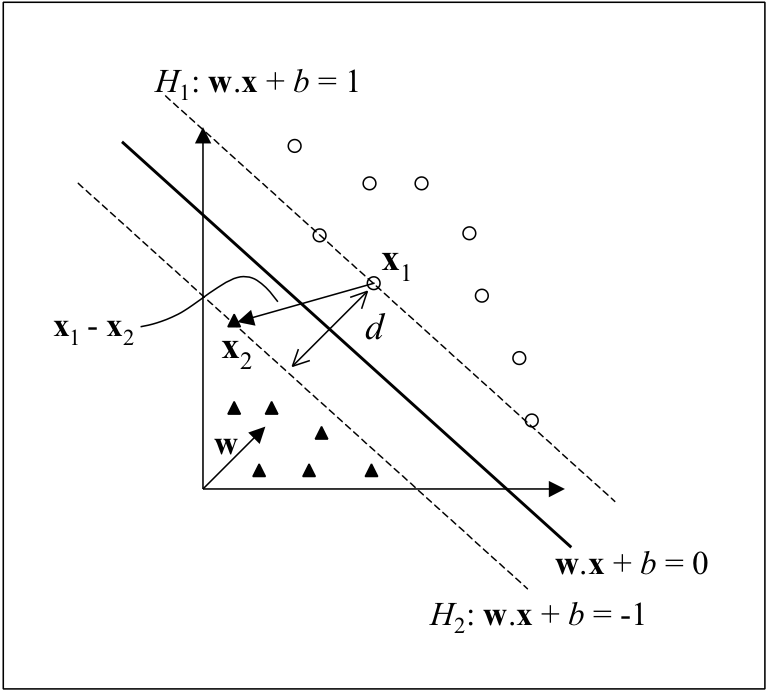
\includegraphics[width=0.5\textwidth]{img/fig-hiperplanos.png}
  \figinfox{Hiperplano separador e margens}{LORENA, 2003}
  \label{fig:hiperplanos}
\end{figure}

Como um dos objetivos do problema de otimização é obter uma margem larga entre os exemplos, pode-se restringir a busca por $\vect{w}$ apenas em termos do cálculo do tamanho da margem. Para isso, é necessário calcular a distância entre dois hiperplanos que são formados pelos exemplos $\vect{x}_1$ e $\vect{x}_2$. Sejam $H_1: \vect{w}\cdot\vect{x} + b = +1$ e $H2: \vect{w}\cdot\vect{x} +b = -1$ dois hiperplanos que ficam paralelamente acima e abaixo, respectivamente, do hiperplano separador. Além disso, assume-se que $H_1$ passa por $\vect{x}_1$ e $H_2$ passa por $\vect{x}_2$. A figura \ref{fig:hiperplanos} mostra a relação entre os hiperplanos e os pontos $\vect{x}_1$ e $\vect{x}_2$.

Conhecendo os hiperplanos, agora é possível calcular a distância entre os hiperplanos que servem de fronteira entre cada ponta da margem do hiperplano separador. A equação \ref{eq:projecao_w} apresenta o cálculo necessário para projetar $\vect{x}_1 - \vect{x}_2$ na direção de $\vect{w}$, que é perpendicular ao hiperplano separador $\vect{w}\cdot\vect{x} + b = 0$.
\begin{equation}\label{eq:projecao_w}
  (x_1 - x_2)
    \left(
      \frac{ \vect{w} }{ \norma{\vect{w}} }
      \cdot
      \frac{(x_1 - x_2)}{ \norma{\vect{x}_1 - \vect{x}_2} }
    \right)
\end{equation}

Sabendo que $\vect{w}\cdot\vect{x}_1 + b = +1$ e $\vect{w}\cdot\vect{x}_2 + b = -1$, e levando em conta que deseja-se saber o comprimento do vetor resultante, é usada a norma da equação \ref{eq:projecao_w} para chegar à equação \ref{eq:projecao_w2}, que indica a distância $d$ utilizada na figura \ref{fig:hiperplanos}:
\begin{equation}\label{eq:projecao_w2}
  d = \frac{2}{\norma{\vect{w}}}
\end{equation}

Portanto, as distâncias entre $\vect{x}_1$, $\vect{x}_2$ e o hiperplano separador $\vect{w}\cdot\vect{x} + b = 0$ são $\frac{1}{\norma{\vect{w}}}$, e com isso, é possível definir o problema de otimização como definido pelo problema de otimização da equação \ref{eq:max_w0}. A restrição \ref{eq:max_w1} indica que $H_1$ e $H_2$ devem passar, respectivamente, pelos vetores $\vect{x}_1$ e $\vect{x}_2$.
\begin{eqnarray}
& \label{eq:max_w0}\operatorname{Maximizar} & \frac{2}{\norma{\vect{w}}} \\
& \label{eq:max_w1} \operatorname{sujeito\;a} & y_i(\vect{w}\cdot\vect{x}_i + b) - 1 \ge 0 \quad i = 1,\dotsc,n.
\end{eqnarray}

No problema de maximização da equação \ref{eq:max_w0}, $\frac{2}{\norma{\vect{w}}}$ pode ser descrito como um problema de minimização de $\norma{\vect{w}}^2/{2}$:
\begin{eqnarray}
& \label{eq:min_w0}\operatorname{Minimizar} & \frac{\norma{\vect{w}}^2}{2} \\
& \nonumber \operatorname{sujeito\;a} & y_i(\vect{w}\cdot\vect{x}_i + b) - 1 \ge 0 \quad i = 1,\dotsc,n.
\end{eqnarray}

%% FIXME rev Neusa: Que função é essa? [função de lagrange] Pelo menos deve colocar uma referência

A partir deste ponto, o problema da equação \ref{eq:min_w0} pode ser resolvido com técnicas de programação quadrática (PQ) \cite{osuna1997support}. Este tipo de problema pode ser solucionado utilizando uma função Lagrangiana e adicionando as restrições à função objetivo junto com os multiplicadores de Lagrange $\alpha_i$ \cite{smola2000advances} (a técnica conhecida como “multiplicadores de Lagrange” tem como objetivo simplificar a busca pelo ponto ótimo de um problema de otimização unindo a função objetivo às funções de restrição). A equação \ref{eq:lagrange0} deve ser minimizada, o que significa maximizar $\alpha_i$ e minimizar $\vect{w}$ e $b$. O problema é representado desta forma para que a restrição (da equação \ref{eq:max_w1}) possa ser representada na forma dos multiplicadores $\alpha_i$, o que facilita os cálculos mais adiante, e também porque os dados de treinamento apenas aparecem na forma de produtos entre vetores \cite{burges1998tutorial}, o que permite o uso de \emph{kernels} (seção \ref{sec:naolinear}).
\begin{equation}\label{eq:lagrange0}
  L(\vect{w}, b, \vect{\alpha}) = \frac{1}{2}\norma{\vect{w}}^2 - 
       \sum_{i=1}^n{\alpha_i(y_i(\vect{w}\cdot\vect{x}_i + b) - 1)}
\end{equation}

Tem-se ponto de sela, então:
\begin{eqnarray}\label{eq:sela}
  \frac{\partial{L}}{\partial{b}} = 0 & \text{e} & \frac{\partial{L}}{\partial{\vect{w}}} = 0
\end{eqnarray}
E com isso:
\begin{eqnarray}
&  \label{eq:lagsum0}  \sum_{i=1}^n{\alpha_i y_i} = 0 \\
&  \label{eq:lagsum1}  \vect{w} = \sum_{i=1}^n{\alpha_i y_i\vect{x}_i}
\end{eqnarray}

Assim, substituindo equações \ref{eq:lagsum0} e \ref{eq:lagsum1}, é possível formular o problema de otimização:
\begin{eqnarray}\label{eq:maxalpha}
\begin{array}{rl}
   %\operatorname*{Maximizar}_{\alpha}
   \underset{\alpha}{\operatorname{Maximizar}}
   & \sum_{i=1}^n{\alpha_i - \frac{1}{2}}
                            \sum_{i,j=1}^n{\alpha_i\alpha_j y_i y_j(\vect{x}_i\cdot\vect{x}_j)} \\
\operatorname{sujeito\;a} &
  \begin{cases}
    \alpha_i \geqslant 0, \forall{i} = 1,\dotsc,n \\
    \sum_{i=1}^n{\alpha_i y_i} = 0
  \end{cases}
\end{array}
\end{eqnarray}

A equação \ref{eq:maxalpha} é denominada a forma dual do problema, ao passo que a formulação original (equação \ref{eq:min_w0}), é denominada a forma primal, baseada no trabalho de \apudonline{fletcher1987practical}{burges1998tutorial}. Chama-se de forma dual a disposição do problema de otimização que envolve os mesmos coeficientes, mas são dispostos de maneira diferente do problema original (chamada de primal), formando um problema que tem ponto ótimo próximo ao da formulação original~\cite{puccini1990introducao}.

% TODO REV Marcio pg16, "quais são as condições [de KKT]"

É possível utilizar as condições Karush-Kuhn-Tucker (KKT), que indicam em quais situações um problema de otimização pode garantidamente chegar a um ponto ótimo, descritas em \citeonline[proposição 3.3.1]{bertsekas-nonlinear}, visto que o problema de otimização \ref{eq:maxalpha} possui restrições lineares e a função objetivo é convexa \cite{burges1998tutorial}. Assim, segundo essas condições, é possível encontrar $\vect{w^*}$ e $b^*$ que podem ser considerados solução ótima para o problema a partir da solução do problema dual ao encontrar $\alpha_i^*$:
\begin{equation}\label{eq:dualalpha}
  \alpha_i^*(y_i(\vect{w^*}\cdot\vect{x}_i+b^*) - 1) = 0, \forall{i}=1,\dotsc,n
\end{equation}

Na equação \ref{eq:dualalpha}, $\alpha_i^*$ é diferente de zero apenas para os valores que tocam a borda das margens do hiperplano de decisão ($H_1$ e $H_2$). Assim, esses dados são chamados de ``vetores de suporte'', pois são os dados mais significativos para a localização de hiperplano $\vect{w}\cdot\vect{x} + b = 0$.

E para calcular $b^*$, de acordo com com a equação \ref{eq:dualalpha}:
\begin{equation}
  b^* = \frac{1}{n_{SV}}\sum_{x_j \in SV}{\frac{1}{y_j} - \vect{w^*}\cdot\vect{x}_j}
\end{equation} Onde $n_{SV}$ é o número de vetores de suporte e $SV$ o conjunto dos mesmos.

% ALELUIA!!!!!!!!!!!! PQPQPQPQPQPQPQP!!!
Finalmente, obtém-se a seguinte função classificadora:
\begin{equation}\label{eq:classificadora}
  g(\vect{x}) = \operatorname{sinal}(f(\vect{x}))
              = \operatorname{sinal}\left(
                  \sum_{x_i \in SV}{y_i\alpha_i^*\vect{x}_i\cdot\vect{x}+b^*}
                \right)
\end{equation}

\subsubsection{Margens suaves}

% seção está incompleta, não explica bem como o erro é tratado em si

Para tratar os casos em que há \emph{outliers} nos exemplos, ou seja, dados que estão rotulados incorretamente ou com algum ruído, utiliza-se a técnica de margens suaves, que é uma saída mais simples que SVMs não-lineares \cite{burges1998tutorial}.

%% TODO FIXME rev Neusa, no trecho "mais simples que SVMs não-lineares": "qual é a complexidade de SVMs não lineares"?

Utiliza-se variáveis de folga $\xi_i$ para cada exemplo $\vect{x}_i$ do conjunto de treinamento. Essas variáveis são adicionadas à restrição do problema primal:
\begin{equation}\label{eq:restrsuave}
  y_i(\vect{w}\cdot\vect{x}_i+b) \geqslant 1 - \xi_i,\quad\forall{i}=1,\dotsc,n
\end{equation}

Ao passo que a função objetivo é reformulada como:
\begin{equation}
  \underset{\vect{w}, b, \vect{\xi}}{\operatorname{Minimizar}}\quad
         \frac{1}{2}\norma{\vect{w}}^2+C\left(\sum_{i=1}^n{\xi_i}\right)
\end{equation}

A constante $C$ impõe uma penalização à violação das restrições descritas na equação \ref{eq:restrsuave} do problema de otimização. O valor desta constante é definida pelo usuário e sua definição depende de testes baseados no conjunto de treinamento. Algumas abordagens para a escolha deste parâmetro foram apresentadas por \citeonline{chapelle2002choosing}, \citeonline{cherkassky2004practical}, \citeonline{quang2002evolving} e \citeonline{ben2010user}.

% FIXME descrever o método de busca em grade de ben2010user, pois é o que
% usamos

\subsubsection{Classificação não-linear}\label{sec:naolinear}

Segundo o teorema de \citeonline{cover1965geometrical}, as chances de que um conjunto de exemplos não linearmente separável possa ser separado por um hiperplano é grande quando este é disposto em um espaço de maior dimensionalidade. Assim, a implementação de SVMs utiliza esta técnica para conseguir separar dados ainda de maneira linear~\cite{burges1998tutorial}.

Com isso, os dois vetores $\vect{x}$ e $\vect{x}_i$, que são utilizados na função de decisão (equação \ref{eq:classificadora}), são convertidos para o espaço de maior dimensão por um mapeamento $\vect{\Phi}: X \rightarrow \Im$, aonde $X$ é o espaço de entrada e $\Im$ o espaço de características.

Adicionalmente, o produto entre os vetores $\vect{x}$ e $\vect{x}_i$ é representado como uma função $K(\vect{x}_i, \vect{x}_j) = \vect{\Phi}(\vect{x}_i)\cdot\vect{\Phi}(\vect{x}_j)$. Esta função é chamada de \emph{função kernel} e tem por finalidade permitir o uso de funções que atentem às condições definidas pelo teorema de Mercer \cite[p. 141]{burges1998tutorial}. Esta forma de representação permite que se use estas funções de kernel dentro da implementação de uma SVM sem a necessidade de conhecimento dos detalhes internos das mesmas. O quadro \ref{quadro:kernels} apresenta alguns dos kernels mais populares utilizados com SVMs~\cite{lorena2003introducaoas}.

\begin{table}[htp]
\centering
\hspace{-2cm} % FIXME arrumar no template
\quadro{Funções de kernel comumente usadas}\label{quadro:kernels}
\begin{tabular}{|c|c|c|}
\hline
Tipo de kernel & Função & Parâmetros \\
\hline
Polinomial & $(\delta(\vect{x}_i\cdot\vect{x}_j)+\kappa)^d$ & $\delta$, $\kappa$, e $d$ \\
Gaussiano (ou RBF) & $\exp(-\sigma\norma{\vect{x}_i-\vect{x}_j}^2)$ & $\sigma$ \\
Sigmoidal & $\tanh(\delta(\vect{x}_i\cdot\vect{x}_j)+\kappa)$ & $\delta$ e $\kappa$ \\
\hline
\end{tabular} \end{table}

\subsubsection{Classificação multiclasses}\label{sec:svmmulti}

% hsu2002comparison

Como SVMs fazem classificação binária, é necessário o uso de alguma técnica para adaptar problemas de classificação multiclasses. As mais populares são um contra todos (\emph{one-against-all}) e um contra um (\emph{one-against-one}).

Na técnica um contra todos, uma SVM é treinada para cada classe contra todas as outras classes ao mesmo tempo. \citeonline{vapnik1998statistical} propôs uma extensão a esta técnica para utilizar os valores contínuos de cada SVM (ao invés do retornado por $\operatorname{sinal}$) e ordenar as classes descendentemente de acordo com o módulo da classificação de cada uma~\cite{abe2003analysis}.

Na técnica de classificação um contra um, também chamada de \emph{pairwise}, cada classe é treinada contra outra classe do problema, sendo a classe selecionada a que foi selecionada mais vezes nas classificações contra todas as outras classes. Isso resulta, em um problema de classificação de $n$ classes, em $n(n - 1)/2$ SVMs \cite{kressel1999pairwise}.

% TODO há mais técnicas interessantes (as baseadas em árvore de decisão e
% all-together), talvez apontar desempenho delas etc etc

%%\subsubsubsection{Complexidade computacional}
%% tratar

%%\subsubsubsection{Implementações}
% abandonada por falta de tempo, vamos citar apenas a libsvm na metodologia
% libsvm 
% PyML
% svm-light
% svm-perf



\section{Virtualização}\label{sec:virt}

O conceito clássico de virtualização consiste na execução simulada de cada
instrução de uma determinada arquitetura bem como a emulação de seu
hardware original, de maneira a permitir que qualquer sistema operacional
compatível possa executar também neste ambiente~\cite{goldberg1974survey}.
Diferentemente do que se observa na arquitetura clássica de computadores,
aonde cada componente provê uma abstração os componentes mais próximos do
usuário, a virtualização multiplexa os serviços de hardware para
componentes virtuais, que possam ser utilizandos por sistemas operacionais
sem adaptações XXX. % FIXME citar os br da 'revisao de virtualizacao'

% FIXME colocar aqui uma figura mostrando uma arquitetura com virtualização

Atribui-se ao sistema \emph{OS/360} a introdução do conceito de
virtualização, que neste caso era limitada a apenas uma instância de uma
\emph{máquina virtual} para os processos não-privilegiados. Com o passar do
tempo isto foi aprimorado com o desenvolvimento dos \emph{Monitores de
Máquinas Virtuais} (também conhecidos como hipervisores ou
\emph{hypervisors}), que eram softwares especializados em executar um
conjunto de instruções de alguma arquitetura e que permitiam então, por
estar não relacionado a um serviço de sistema operacional, executar
múltiplas máquinas virtuais, permitindo assim que o custo computacional com
a execução simulada das instruções fosse compensado com a execução de
muitas máquinas virtuais, aproveitando assim o tempo de
CPU~\cite{goldberg1974survey}.

Com a popularização da internet e o barateamento do hardware, a
virtualização começou a ser utilizada com o intuito de facilitar a
manutenção em ambiente de servidores. A facilidade da criação e
configuração permitiu que serviços executem em máquinas (virtuais)
dedicadas, aumentando a segurança (por meio do isolamento) e facilitando a
manutenção com menor risco de comprometimento de outros
serviços~\cite{smith2005architecture}.

% FIXME citar aqui introdução do conceito de cloudcomputing

% FIXME começar a descrever tolerância a faltas, e então descrever migração
% e as tais técnicas de sincronização de blabla

% FIXME remover essa porcaria
É importante apresentar alguns conceitos que são amplamente utilizados ao
tratar de virtualização, como apresentado por
\citeonline{peter2005resource}:
\begin{description}
  \item[hóspede] refere-se à máquina virtual;
  \item[hospedeiro] refere-se ao Monitor de Máquinas Virtuais;
  \item[paravirtualização] conjunto de técnicas no qual o hóspede oferece
        serviços ao hospedeiro, que por sua vez possui suporte explícito a
        eles;
  \item[migração] ocorre quando todo o estado de um hóspede
       (memória, registradores, dispositivos) que está executando em um
       determinado hospedeiro é transfeirido para outro, de maneira que a
       execução do hóspede prossegue, sem que software executando dentro
       desta note diferença.
\end{description}

\subsection{Ferramentas}

Atualmente existe uma grande diversidade de ferramentas que atuam como
monitores de máquinas virtuais. Algumas utilizam implementações de
virtualização utilizando técnicas mais simples e com maior custo
computacional, ao passo que outras são mais sofisticadas, além do uso de
recursos de virtualização disponíveis em CPUs modernas.

A família de produtos oferecida pela empresa VMWare está entre as mais
populares ferramentas de virtualização utilizadas atualmente. Seu primeiro
produto lançado, o \emph{VMWare Workstation}, que foi lançado em
1999~\cite{vmwareMilestones}, que tornou-se popular em razão de seu bom
desempenho resultante do uso de técnicas de tradução binária dinâmica.

Além disso, uma outra ferramenta muito popular para virtualização é a
VirtualBox.

% mais ferramentas interessantes: bochs, denali, ibm rhype, virtualbox

% introdução
% ferramentas

% descrição de medidas de carga de CPU: loadavg e percentual de uso de CPU

\subsection{\libvirt}\label{sec:libvirt}

% uma descrição mais detalhada, 
% virt-manager
% virsh
% "conceitos"

A \libvirt{} é um conjunto de ferramentas que visa prover uma abstração
uniforme para gerenciamento de máquinas virtuais de maneira independente da
da aplicação de virtualização que está sendo utilizada. Seu desenvolvimento
foi iniciado em 2005 pela empresa Red Hat e inicialmente chamava-se
\emph{libxen} (indicando assim que era uma abstração específica para a
ferramenta \emph{Xen}), porém teve seu nome alterado para \libvirt{} em
2006, de maneira a refletir o interesse em suportar mais ferramentas de
virtualização \apud{gitlibvirt}{eriksson2009virtualization}.

\subsubsection{Interface de programação}\label{sec:libvirtapi}

\emph{Trecho ainda não concluído}.


%
% Trabalhos relacionados
%

\chapter{Trabalhos relacionados}

Pode-se observar que a área que possui uma grande quantidade de artigos
relacionados ao problema de tentar prever o uso de CPU é a de sistemas
distribuídos. Isso se deve ao fato de que em certos tipos de sistemas
distribuídos, é necessário que tarefas sejam despachadas para execução por
unidades de processamento que, preferencialmente, estejam ociosas~\cite{zhang2007cpu}.

Os trabalhos de Dinda (2000)\nocite{dinda2000host} e de Dinda
(2002)\nocite{dinda2002evaluation} efetuam a coleta de informações de uso de
CPU em um conjunto formado por 38 computadores de diferentes tipos que
pertenciam ao \emph{Carnegie Mellon University} e também no \emph{Pittsburgh
Supercomputing Center}, nos Estados Unidos, pelo período de pouco mais que uma
semana. Com estas informações de uso de CPU foi feita uma análise deste conjunto
de dados e avaliou-se algumas técnicas de modelagem de séries temporais, e
finalmente sugere que seja usado o modelo AR(16) (\emph{Autoregressive model},
modelo auto-regressivo, com 16 coeficientes) para a predição de comportamento
de CPUs. Este modelo consiste em uma representação na forma
$x_t = \phi_{1}x_{t-1} + \phi_{2}x_{t-2}+\dotsc,\phi_{p}x{t-p}+e_t$, aonde a
$\phi_p$ correspondem aos parâmetros do modelo (sendo $p$ a ordem do mesmo) e
$e_t$ representa um ruído no modelo. Utilizando a técnica de Yule-Walker é
possível conhecer os parâmetros $\phi_p$ do modelo e assim prever itens na
série calculando-se $x_{t+1}$~\cite{baddour2005autoregressive}.

% tese do eugeni
% dinda (análise de comportamento dos hosts, virtuoso)
% skeletons
% homeostatic,
% etc


%
% Metodologia
%
%
% - diagramas de contexto descrevendo quais serão as informações de
%   entrada, qual módulo do software fará o processamento e como serão
%   disponibilizadas as informações da predição,
% - diagrama de classes para a implementação do software,
% 
% - descrição de quais técnicas serão utilizadas e como serão implementadas,
% - descrição de um protocolo para avaliação do desempenho das técnicas
% implementadas.
%
%

\chapter{Metodologia de desenvolvimento}\label{sec:meto}

\section{Introdução}

% Em um ambiente de virtualização gerenciado pela ferramenta \libvirt{}
% (apresentada na seção \ref{sec:libvirt}), o software executará em plano de
% fundo (ou seja, será um \emph{daemon}) e estará periodicamente coletando
% informações quantitativas a respeito do tempo de uso de processador de
% cada uma das máquinas virtuais que fazem parte de um determinado
% \emph{domínio}. Este utilizará tais informações para treinar um
% mecanismo de aprendizado de máquina. Utilizando este mecanismo, a
% ferramenta poderá então prever em quais situações alguma máquina virtual
% exigirá mais uso de processador que a máquina \emph{host} em que ela
% executa terá condições de atender sem prejudicar as outras.

A figura \ref{fig:hostguests1} apresenta um ambiente de virtualização
mínimo, onde tem-se um computador, denominado \texttt{host}, que está
hospedando três máquinas virtuais \texttt{mv-1}, \texttt{mv-2} e
\texttt{mv-3}. Estas máquinas virtuais estão sendo gerenciadas por qualquer
uma das ferramentas que são suportadas pela \libvirt{}, e cada uma delas
pode estar executando qualquer sistema operacional, e nestes podem estar
executando qualquer tipo de software, mais comumente servidores de banco de
dados e aplicações Web.

\begin{figure}[htp]
\centering
\includegraphics{img-host-guests1.pdf}
\figinfo{Ambiente com um hospedeiro e poucos hóspedes}
\label{fig:hostguests1}
\end{figure}

Se o indivíduo que criou este ambiente esperava que as aplicações que
executam dentro das máquinas virtuais tenham um desempenho aceitável,
então ele deve ter estudado os usos de processador, memória e entrada/saída
dessas aplicações e dimensionado o ambiente de tal maneira que uma máquina
virtual não degrade o desempenho de outra a ponto de torná-lo inaceitável.

\begin{figure}[htp]
\centering
\includegraphics{img-host-guests2.pdf}
\figinfo{Ambiente com vários hospedeiros e hóspedes}
\label{fig:hostguests2}
\end{figure}

Porém, à medida que mais máquinas virtuais forem necessárias, como é
apresentado na figura \ref{fig:hostguests2}, novas máquinas físicas terão
que ser alocadas para acomodar as novas demandas. E a partir deste ponto
gerenciar este parque computacional começa a tornar-se uma tarefa
desafiadora, pois é necessário tentar acomodar tais máquinas virtuais
levando em conta as necessidades particulares de cada aplicação que estão
executando nelas.

\begin{figure}[htp]
\centering
\includegraphics{img-host-guests3.pdf}
\figinfo{Dois hospedeiros e carga de CPU aceitável das MVs}
\label{fig:hostguests3}
\end{figure}

Na figura \ref{fig:hostguests3}, a máquina \texttt{host3} possui cinco máquinas
virtuais que ocupam, ao todo, 57\% do tempo de processamento. Se estas
máquinas virtuais mantiverem o mesmo comportamento no decorrer do tempo de
vida deste ambiente, a única mudança necessária seria de talvez desligar
\texttt{host1} e migrar estas máquinas virtuais para \texttt{host3}, já que
este hospedeiro ainda tem aproximadamente 43\% de tempo de processamento
sendo desperdiçado. Sendo \texttt{host1} desligada, haveriam menos custos
com energia e manutenção.

Porém, os serviços que executam nestas máquinas virtuais podem sofrer um
abrupto aumento de demanda, o que é mais ainda provável em aplicações que
estão acessíveis por meio da Internet, como servidores web, ou serviços
relacionados, como servidores de banco de dados. Nestes casos, o
administrador do ambiente precisa provisionar rapidamente recursos para
atender a essa demanda.

\begin{figure}[htp]
\centering
\includegraphics{img-host-guests4.pdf}
\figinfo{Dois hospedeiros e carga das MVs desbalanceada entre eles}
\label{fig:hostguests4}
\end{figure}

No exemplo da figura \ref{fig:hostguests4}, a máquina virtual
\texttt{vm-11} está executando algum processo que está exigindo muito tempo
de CPU. Este tipo de situação pode ocorrer quando há este processo é
\emph{CPU-bound} (que faz uso intensivo do processador), o que geralmente
pode ser uma tarefa rotineira de \emph{backup} (compressão, descompressão ou
sincronização de árvores) ou o rotinas aritméticas. Neste caso fica claro que
seria melhor ter esta máquina executando no hospedeiro \texttt{host1}, pois o
uso típico de CPU das máquinas virtuais que já estão lá ainda pode acomodar
\texttt{vm-11}. A dificuldade neste modelo está no fato de que este uso de CPU
pode ser sazonal, e que outras máquinas virtuais além de \texttt{vm-11} podem
ter situações de demanda abrupta.

Com isso, o software que será desenvolvido a partir deste projeto atuará
tentando prever o comportamento destas máquinas virtuais e requisitando à
ferramenta de virtualização que migre aquelas que apresentarem perspectiva
de uso intensivo de CPU para um hospedeiro que tenha condições de tratar
aquela demanda. Ele executará como um processo separado, na forma de um
\emph{daemon} (que estará executando como serviço do sistema). Este poderá
estar instalado em qualquer uma das máquinas hospedeiras ou até mesmo em
uma máquina separada (providas as credenciais de acesso para a \libvirt{}).

\begin{figure}[htp]
\centering
\includegraphics{img-libvirt-contexto0.pdf}
\figinfo{Interação entre \libvirt{} e projeto}
\label{fig:libvirtcontexto0}
\end{figure}

De maneira a ser útil para o maior número de usuários de ferramentas de
virtualização, este projeto utilizará a ferramenta \libvirt{} como
interface para controle e migração das máquinas virtuais, pois esta possui
suporte às principais softwares disponíveis atualmente, como descrito na
seção \ref{sec:libvirt}. A figura \ref{fig:libvirtcontexto0} descreve de
maneira superficial como será a interação entre o software a ser
implementado e a \libvirt{}. O software estará periodicamente coletando
informações a respeito de uso de CPU das máquinas virtuais sendo
gerenciadas (1). E com essas informações, o software fará predições a
respeito do comportamento destas máquinas virtuais e então enviará comandos
por meio da API (\emph{Application Programming Interface}, Interface de
Programação de Aplicação) da \libvirt{} (2), comandos estes indicando qual
máquina virtual deve migrar para qual máquina hospedeira. A \libvirt{} por
sua vez comunicará a ferramenta de virtualização (3) que então executará a
migração entre um hospedeiro e outro (4).

% colocar aqui um ou mais diagramas descrevendo as máquinas virtuais que
% estão em um ambiente "folgado" e então indicar uma situação em que uma
% máquina virtual precisa ser migrada e daí migrar para outra máquina.

\section{Modelagem do software}\label{sec:modelagem}

\begin{figure}[htp]
\centering
\includegraphics{img-met-contexto-0.pdf}
\figinfo{Diagrama de contexto, interação entre as principais entidades no
sistema}
\label{fig:contexto0}
\end{figure}

A figura \ref{fig:contexto0} apresenta um diagrama de contexto, de nível 0,
indicando a relação entre o projeto que será desenvolvido e a biblioteca
\libvirt{}. O fluxo \texttt{estatísticas das máq. virtuais} indica as
informações a respeito de uso de CPU que são providas pela libVirt,
enquanto que \texttt{cmds. de migração} indica os comandos, transmitidos
por meio da API (introduzida na seção \ref{sec:libvirtapi}), que são enviadas
à \libvirt{} para a migração das máquinas virtuais, de acordo com o que o
software a ser implementado decidir.

\begin{figure}[htp]
\centering
\includegraphics{img-met-contexto-1.pdf}
\figinfo{Diagrama de contexto, nível 1, interação entre os processos do
projeto proposto}
\label{fig:contexto1}
\end{figure}

Como o projeto será implementado utilizando o conceito de orientação a
objetos~\cite{ricarte2001programacao}, a figura \ref{fig:contexto1} maximiza o
processo \texttt{Projeto} utilizando um diagrama de
classes~\cite{bezerra2002principios} descrevendo quais são os processos que
fazem parte do software proposto. O fluxo \texttt{uso de CPU máq. virtuais}
(também abreviado como \texttt{usos de CPU}) indica os valores que serão lidos
periodicamente de cada máquina virtual.  O processo \texttt{Coleta} trata da
consulta à instância da \libvirt{} e o pré-processamento dos dados para envio à
base. O processo \texttt{Treinamento} será executado periodicamente e
consistirá na execução da fase de treinamento para as técnicas de AM
(aprendizado de máquina). O depósito de dados \texttt{base ``treinada''}
representa uma base de dados com os parâmetros utilizados para representar o
conhecimento dos algoritmos de AM (o conteúdo em si desta base depende
da técnica utilizada; SVMs, por exemplo, guardam alguns exemplos da base de
treinamento, já $k$-NN não guarda coisa alguma além dos exemplos). O processo
\texttt{Predição} recebe dois fluxos de dados, o primeiro é o das informações
de treinamento da \texttt{base ``treinada''}, o segundo é das mesmas
informações de CPU que vieram da etapa \texttt{Coleta}; este processo utiliza o
algoritmo de aprendizado para saber se alguma das máquinas virtuais que estão
sendo monitoradas tem possibilidade de saturar os recursos de processador das
máquinas hospedeiras; é esse processo que envia os comandos necessários à
\libvirt{} visando migrar máquinas para outro hospedeiro que possa acomodá-lo.

% FIXME explicar esse tal pré-processamento

\begin{figure}[htp]
\centering
\includegraphics{img-diagrama-classes0.pdf}
\figinfo{Diagrama das principais classes do software proposto}
\label{fig:diagramaclasses0}
\end{figure}

Na figura \ref{fig:diagramaclasses0} é apresentado um diagrama com as
principais classes do software. A classe \texttt{Projeto} representa uma
instância de todo o projeto e também é responsável pelo controle do ciclo
de vida das classes que fazem coleta, aprendizado e predição. Cada uma
destas classes possui apenas um método público, para que estes sejam
chamados apenas quando a classe \texttt{Projeto} considerar conveniente,
fazendo com que assim esta classe tenha um papel de escalonador do
software. As classes são a grosso modo um mapeamento dos processos
apresentados na figura \ref{fig:contexto1}, com exceção da classe
\texttt{InterfaceMMV}, que significa Interface para Monitor de
Máquinas Virtuais, tem como propósito centralizar o acesso à \libvirt{},
facilitando a manutenção em caso de mudança de interface, porte para outra
biblioteca ou a simulação de valores (que é descrita na seção
\ref{sec:desemp}). À exceção de \texttt{InterfaceMMV}, todas estas
classes são abstratas, pois devem ainda ser especializadas para cada uma
das técnicas de aprendizado que serão implementadas no projeto.

% diagrama de classes

\section{Metodologia de avaliação das técnicas}

Para as etapas de aprendizado e predição, serão utilizados os métodos de
aprendizado de máquina \emph{Support Vector Machines} (Máquinas de Vetores
de Suporte) e $k$-NN ($k$-\emph{Nearest Neighbors}). A primeira em razão de seu
bom desempenho em diversos tipos de problemas de aprendizado, como em
detecção de escrita, reconhecimento de faces, categorização de texto, e
outras~\cite{bennett2000support}. $k$-NN foi escolhido por se tratar de uma
técnica, que em alguns casos, pode ter desempenho melhor que técnicas
sofisticadas, servindo como base e indicação de quando uma técnica pode
estar mal implementada, como indicado por \citeonline{joachims1998text} e
\citeonline{hafner2007comparison}.

Assim, das classes que foram apresentadas na seção \ref{sec:modelagem},
serão especializações para cada tipo de técnica de aprendizado. O diagrama
representando estas especializações é apresentado na figura
\ref{fig:diagramaclasses1}.

\begin{figure}[htp]
\centering
\includegraphics{img-diagrama-classes1.pdf}
\figinfo{Diagrama com classes especializando cada tipo de aprendizado
utilizado}
\label{fig:diagramaclasses1}
\end{figure}

% Para o caso de SVMs, será usada a técnica de um-contra-todos (descrita na seção
% \ref{sec:svmmulti}), que consiste na criação múltiplas instâncias de SVM,
% representando a identificação de uma classe.

Para o caso de SVMs, este trabalho seguirá a metodologia proposta
por~\citeonline{hsu2003practical} para a avaliação dos parâmetros que serão
utilizados no sistema. Esta consiste na execução nos seguintes passos:
\begin{enumerate}
  \item processar os dados coletados para transformar no formato da biblioteca
        que será utilizada (no caso, a \emph{libsvm});
  \item normalizar os dados;
  \item avaliar o desempenho do uso da função \emph{kernel} RBF
        ($\exp(-\sigma\norma{\vect{x}_i-\vect{x}_j}^2)$);
  \item fazer busca em grade: dos valores do espaço de busca, crescendo os
	 parâmetros da SVM e da função de kernel ($C$ e $\sigma$,
         respectivamente) exponencialmente;
  \item executar testes de validação cruzada (intercalando elementos do conjunto
        de testes com o de treinamento);
 \item avaliar o desempenho na base de dados completa;
\end{enumerate}

\subsection{Treinamento}

Para a etapa de treinamento, e subsequente uso pela etapa de predição, o
vetor de características usado será constituído de uma janela
formada por um determinado número de leituras anteriores do uso de CPU para
cada máquina virtual controlada naquele domínio. Como estes valores são
percentuais de uso de CPU, a normalização destes será feita com uma divisão
de cada valor por $100$.

Para a classe usada em cada exemplo do treinamento, serão utilizados
valores categóricos. Cada classe representará uma faixa de valor do
percentual de uso de CPU. Por exemplo, a faixa 0--24\% seria a classe
\texttt{A}, 25--49\% a classe \texttt{B}, e assim por diante.

\begin{figure}[htp]
\centering
\includegraphics{img-vetor0.pdf}
\figinfo{Exemplo de série de valores lida e composição do vetor de
características}
\label{fig:vetor0}
\end{figure}

Na figura \ref{fig:vetor0}, o item \emph{(a)} apresenta uma janela
formada por valores lidos da série para uma máquina virtual. Em \emph{(b)}
são apresentados os vetores de características que são usados para treinar
(para os testes que usarão SVMs) cada uma das SVMs usadas para categorizar
o uso de CPU. Para este exemplo há 4 classes, o valor $1$ representa a
classe selecionada, e $-1$ a não-seleção dela.

Além disso, serão feitos testes com vetores de características contendo
informações a respeito do período do dia, e dia da semana, de maneira a
tentar capturar características sazonais no comportamento das máquinas
virtuais.

\subsection{Predição e migração}

Para a etapa de predição, serão utilizados os métodos de classificação das
técnicas de aprendizado de máquina que foram selecionadas. O resultado da
classificação, para cada máquina virtual, irá consistir em uma faixa de
percentual de uso de CPU para. Esta faixa então será usada para calcular o
potencial uso total de CPU para o próximo intervalo de tempo (intervalo
este que será diferente durante os testes) e então será aplicada a técnica
de \emph{first-fit}~\cite{yao1980new} decidir se uma determinada máquina
virtual deve permanecer ou ser migrada para outra disponível. Opta-se por
utilizar esta técnica de empacotamento em razão desta ser mais conservadora
se comparada a \emph{first-fit decreasing} ou outras técnicas, pois
reordenar a lista de máquinas virtuais pode resultar em desnecessárias
migrações entre hospedeiros.

Após o empacotamento das previsões na lista de hospedeiros, aquelas
máquinas virtuais que não estiverem mais em seus hospedeiros originais
serão efetivamente migrados utilizando a \libvirt{}.

\section{Avaliação de desempenho}\label{sec:desemp}

% utilizar SVM, K-NN, AR(16) (se for fácil de implementar)
% variar o tamanho das janelas de histórico
% utilizar uma instância do classificador para todas as VMs, versus
% utilizar uma instância nova para cada VM

Para avaliar o desempenho do projeto a ser implementado, serão lidos os
valores de uso de CPU de um conjunto de máquinas que fazem parte do
ambiente de compilação de software que é utilizado no projeto
\emph{Mandriva Linux}. Tais valores serão lidos por um período de 30 dias,
com o intuito de cobrir as diferentes taxas de uso de CPU naquele período.

Este ambiente de compilação é composto por $6$ máquinas que recebem
comandos de compilação de pacotes de software, fazem download códigos fonte
compactados, os descompactam, compilam (que na maioria dos casos são em
linguagem C ou C++) e então os binários e arquivos documentação gerados são
arquivados no formato RPM~\cite{ewing1996rpm}. Estas etapas apresentam
momentos com forte acesso à mídias de armazenamento (\emph{I/O-bound}) bem
como momentos de intenso uso de CPU (\emph{CPU-bound}).

\begin{figure}[htp]
\centering
\includegraphics{img-diagrama-classes2.pdf}
\figinfo{Diagrama com classes especializada para simulação e acesso à
\libvirt{}}
\label{fig:diagramaclasses2}
\end{figure}

A leitura destes valores será feita a cada minuto utilizando o utilitário
\emph{top}, que coleta estatísticas de uso de recursos por processos e no
sistema operacional como um todo~\cite{andresen2004monitoring}. Para utilizar
os valores coletados no ambiente de compilação, será criada uma especialização
para a classe \texttt{InterfaceMMV}, como descrito na figura
\ref{fig:diagramaclasses2}, que lerá os arquivos com o histórico de acesso às
máquinas e então entregará estes valores ao módulo de aprendizado.

Além disso, o software implementado será testado em um ambiente de
virtualização real, onde cada máquina virtual estará executando pequenos
programas que estarão ocupando as CPUs de maneira a simular os
comportamentos observados no ambiente de compilação descrito anteriormente.
Estes programas serão implementados utilizando laços de repetição que
executarão operações simples (também chamados de \emph{busy loops}), como
implementado também por \citeonline{dinda2000realistic}.

Finalmente, serão avaliados diferentes valores em parâmetros utilizados
pelo sistema a ser implementado, a saber:

\begin{itemize}
  \item no caso de $k$-NN, o valor de $k$ será alterado, seguindo as
        recomendações de \citeonline{hall2008choice};
   \item o tamanho da janela usada para treinamento e predição, como sugerido
        por \citeonline{frank2001time};
   \item no caso de SVM, o parâmetros $C$, como descrito por \citeonline{ben2010user};
   \item no caso de simulação sem ambiente completo, o número de hospedeiros disponíveis;
   \item a quantidade de faixas dividindo o percentual de uso de CPU para
         uso no atributo categórico da etapa de classificação;
% o que mais?
\end{itemize}

% FIXME não sei que técnicas usar aqui
% A mudança no valor destes parâmetros serão avaliados por meio das seguintes
% métricas:
% \begin{itemize}
%   \item
%   \item bar
% \end{itemize}

Os resultados para cada combinação de parâmetros serão considerados
aceitáveis ou não de acordo com a aderência aos seguintes o
objetivos/questionamentos:
\begin{itemize}
  \item Em momentos de baixo uso de tempo de CPU, foi possível manter as
        máquinas virtuais em um conjunto menor de hospedeiros? (Permitindo
        assim que estas máquinas entrem em estados de menor consumo de
        energia e menor gasto com manutenção.)
  \item Em momentos de alto uso de CPU, as máquinas virtuais mais ativas
        foram migradas para hospedeiros mais ociosos? (Evitando assim a
        degradação do desempenho em outros processos.)
\end{itemize}

\section{Detalhes de implementação}

O projeto será implementado na linguagem \emph{Python} \cite{rossum1995python}.
Esta possui tipagem dinâmica, suporta o paradigma de orientação a objetos e com
isso facilita a prototipagem de projetos \cite{lutz2006programming}.

O ambiente de desenvolvimento será baseado no sistema operacional Linux
\cite{morimoto2004entendendo}, que é a plataforma principal de
desenvolvimento e teste da \libvirt{}. Mesmo a biblioteca sendo acessível
de qualquer sistema operacional, a proximidade com o ambiente de
desenvolvimento diminui a probabilidade de encontrar incompatibilidade
entre ferramentas durante a fase de implementação. A distribuição Linux
utilizada será \emph{Mandriva Linux}\footnote{http://www.mandriva.com/},
que possui em sua base de pacotes todas as ferramentas necessárias para a
implementação. O pacote \texttt{python-libvirt} será utilizado para acessar
os módulos da \libvirt{}.

Para o monitor de máquinas virtuais será utilizado o
KVM,\footnote{http://linux-kvm.org/} que é de código aberto e também
desenvolvido pela empresa Red Hat, garantindo assim maior compatibilidade
com a \libvirt{}.

Para a implementação das instâncias de SVM, será utilizada a
\emph{libsvm}~\cite{chang2001libsvm}. O motivo da escolha desta
implementação deve-se se em razão de sua licença, que permite uso e
distribuição, incluindo uso comercial.


\chapter{Conclusão}

Pode-se considerar que o objetivo deste trabalho foi parcialmente atingido. Foi
possível predizer o uso de CPU no ambiente estudado com taxas de acerto a
partir de 98\% utilizando a técnica de máquinas de vetores de suporte com tempo
de execução sem degradar o sistema como um todo.

Além disso, foi possível demonstrar que é possível implementar um software de
consolidação utilizando as técnicas de predição avaliadas e avaliar seu
desempenho através de um simulador. Observou-se que um ambiente com cinco
máquinas reais teve sua carga simulada utilizando, em grande parte do tempo,
apenas duas máquinas hospedeiras

Houve dificuldade, porém, em avaliar o desempenho da ferramenta de consolidação
em um ambiente real, em função da dificuldade de obter uma fonte de informação
apropriada para conhecer quanto tempo de CPU uma máquina virtual realmente
demanda.


%
% Cronograma
%

\chapter{Cronograma}


%
% Glossário
%
\chapter{Glossário}

\begin{description}
\item[KVM] Kernel-based Virtual Machine.
\item[VM] do inglês \emph{Virtual Machine}, Máquina Virtual.
\item[MV] Máquina Virtual.
\end{description}


\bibliography{biblio}

\end{document}
